\documentclass[aspectratio=169]{beamer}
\usepackage{tikz}
\usepackage{graphicx}
\usepackage{listings}
\usepackage{xcolor}
\usepackage{hyperref}
\usepackage[spanish,es-noquoting]{babel}
\usepackage[round]{natbib}

\lstset{
  basicstyle=\ttfamily\small,
  keywordstyle=\color{blue},
  stringstyle=\color{red},
  commentstyle=\color{gray},
  showstringspaces=false
}

% Clean Theme Setup & Optimization
\usetheme{Warsaw}
\usecolortheme{default}
\usefonttheme{serif}

% Remove top headline bar and navigation clutter to maximize slide text space
\setbeamertemplate{headline}{}
\setbeamertemplate{navigation symbols}{}
\setbeamertemplate{frametitle continuation}{}

% Slim, clean footline bar
\setbeamertemplate{footline}{
  \leavevmode%
  \hbox{%
    \begin{beamercolorbox}[wd=.333333\paperwidth,ht=2.25ex,dp=1ex,left]{author in head/foot}%
      \hspace*{2ex}\insertshortauthor
    \end{beamercolorbox}%
    \begin{beamercolorbox}[wd=.333333\paperwidth,ht=2.25ex,dp=1ex,center]{title in head/foot}%
      \insertshorttitle
    \end{beamercolorbox}%
    \begin{beamercolorbox}[wd=.333333\paperwidth,ht=2.25ex,dp=1ex,right]{date in head/foot}%
      \insertframenumber{} / \inserttotalframenumber\hspace*{2ex}
    \end{beamercolorbox}%
  }%
  \vskip0pt%
}

% Font size and list spacing optimizations to prevent text overflow
\setbeamertemplate{itemize/enumerate body begin}{\small}
\setbeamertemplate{itemize/enumerate subbody begin}{\footnotesize}
\setbeamertemplate{itemize/enumerate subsubbody begin}{\scriptsize}

\makeatletter
\g@addto@macro\itemize{%
  \setlength{\itemsep}{2pt}%
  \setlength{\parsep}{1pt}%
  \setlength{\topsep}{2pt}%
  \setlength{\partopsep}{0pt}%
}
\makeatother

\graphicspath{{../}{./}}
\setbeamertemplate{caption}[numbered]

% Title info
\title[Módulo 3]{Módulo 3}
\subtitle{ De colección de prompts a sistema organizacional}
\author{Ricardo Reyes-Jimenez}
\institute{Universidad de La Sabana}
\date{\today}


% Background image for title slide
\usebackgroundtemplate{
  \tikz\node[opacity=0.3]{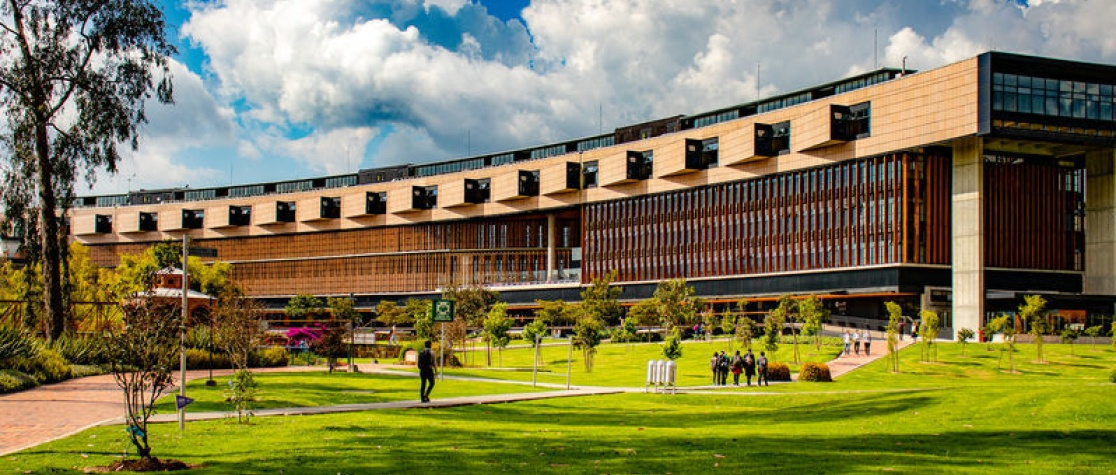
\includegraphics[width=\paperwidth,height=\paperheight]{Images/UniSabana.jpg}};
}


\begin{document}

% Title slide
\begin{frame}
  \titlepage
\end{frame}

% Reset background for normal slides
\usebackgroundtemplate{}


\begin{frame}[allowframebreaks,fragile]{Objetivos de la Sesión}


Al finalizar podrás:

\begin{itemize}
  \item Refinar Blueprints.
  \item Diseñar prompts modulares.
  \item Crear mecanismos de gobernanza.
  \item Definir métricas de éxito.
  \item Escalar una PromptLibrary institucional.
\end{itemize}
\end{frame}

\begin{frame}[allowframebreaks,fragile]{Recapitulación}


Ya tenemos:

\begin{itemize}
  \item Blueprints.
  \item Casos de uso.
  \item Primeras plantillas.
  \item Experiencia práctica.
\end{itemize}
Ahora debemos escalar.

\end{frame}

\begin{frame}[allowframebreaks,fragile]{El Problema de Escalar}


Muchas organizaciones crean:

\begin{itemize}
  \item Exceles.
  \item Documentos compartidos.
  \item Carpetas de prompts.
\end{itemize}
Meses después nadie los usa.

¿Por qué?

Porque carecen de gobernanza.

\end{frame}

\begin{frame}[allowframebreaks,fragile]{Ciclo de Vida de un Blueprint}


\begin{itemize}
  \item Creación.
  \item Prueba.
  \item Retroalimentación.
  \item Refinamiento.
  \item Aprobación.
  \item Publicación.
  \item Auditoría.
\end{itemize}
\end{frame}

\begin{frame}[allowframebreaks,fragile]{La Regla de Oro}


El primer prompt nunca es el definitivo.

Todo Blueprint debe evolucionar.

\end{frame}

\begin{frame}[allowframebreaks,fragile]{Prompt Engineering Jurídico}


La calidad depende de:

\begin{itemize}
  \item Claridad.
  \item Contexto.
  \item Restricciones.
  \item Ejemplos.
  \item Formato.
\end{itemize}
\end{frame}

\begin{frame}[allowframebreaks,fragile]{Técnica Few-Shot}


Consiste en mostrar ejemplos.

En lugar de explicar únicamente:

``Así debe verse el resultado.''

Los modelos aprenden mejor.

\end{frame}

\begin{frame}[allowframebreaks,fragile]{Grounding Jurídico}


Grounding significa:

Anclar la respuesta a fuentes verificables.

Ejemplo:

``Responde únicamente utilizando el texto suministrado.''

\end{frame}

\begin{frame}[allowframebreaks,fragile]{El Problema de las Alucinaciones}


Cuando la IA no tiene evidencia suficiente:

Puede completar vacíos.

Por eso:

\begin{itemize}
  \item Se debe limitar.
  \item Se debe verificar.
  \item Se debe auditar.
\end{itemize}
\end{frame}

\begin{frame}[allowframebreaks,fragile]{Troubleshooting Jurídico}


Si el resultado es malo:

Preguntar:

\begin{itemize}
  \item ¿Faltó contexto?
  \item ¿Faltaron restricciones?
  \item ¿Faltaron ejemplos?
  \item ¿La tarea era demasiado amplia?
\end{itemize}
\end{frame}

\begin{frame}[allowframebreaks,fragile]{Inteligencia Colectiva}


Un prompt mejora cuando:

\begin{itemize}
  \item Varias personas lo prueban.
  \item Diferentes áreas lo utilizan.
  \item Se documentan observaciones.
\end{itemize}
\end{frame}

\begin{frame}[allowframebreaks,fragile]{Del Prompt al Estándar}


No todo prompt entra a la biblioteca oficial.

Debe existir validación.

\end{frame}

\begin{frame}[allowframebreaks,fragile]{¿Qué es un Prompt Modular?}


Un problema complejo se divide en pasos.

La complejidad se reduce.

La precisión aumenta.

\end{frame}

\begin{frame}[allowframebreaks,fragile]{Encadenamiento}


Proceso:

Entrada → Prompt A → Prompt B → Prompt C → Resultado

\end{frame}

\begin{frame}[allowframebreaks,fragile]{Pipeline Contractual}


Etapa 1:

Extracción de cláusulas.

Etapa 2:

Clasificación de riesgos.

Etapa 3:

Priorización.

Etapa 4:

Resumen ejecutivo.

\end{frame}

\begin{frame}[allowframebreaks,fragile]{Pipeline de Litigio}


Etapa 1:

Extracción cronológica.

Etapa 2:

Identificación de pruebas.

Etapa 3:

Contradicciones.

Etapa 4:

Construcción de teoría del caso.

\end{frame}

\begin{frame}[allowframebreaks,fragile]{Niveles de Madurez en IA}


Nivel 1: Uso individual.

Nivel 2: Compartición informal.

Nivel 3: Biblioteca formal.

Nivel 4: Gobernanza.

Nivel 5: Optimización continua.

\end{frame}

\begin{frame}[allowframebreaks,fragile]{Fase 1: Personal}


Herramientas:

\begin{itemize}
  \item Notion.
  \item OneNote.
  \item Word.
  \item Obsidian.
\end{itemize}
Objetivo:

Capturar conocimiento.

\end{frame}

\begin{frame}[allowframebreaks,fragile]{Fase 2: Compartida}


Herramientas:

\begin{itemize}
  \item Teams.
  \item OneDrive.
  \item SharePoint básico.
\end{itemize}
Objetivo:

Colaboración.

\end{frame}

\begin{frame}[allowframebreaks,fragile]{Fase 3: Institucional}


Características:

\begin{itemize}
  \item Catálogo.
  \item Etiquetas.
  \item Aprobaciones.
  \item Auditorías.
  \item Métricas.
\end{itemize}
\end{frame}

\begin{frame}[allowframebreaks,fragile]{Gobernanza de IA}


Preguntas fundamentales:

\begin{itemize}
  \item ¿Quién crea?
  \item ¿Quién aprueba?
  \item ¿Quién modifica?
  \item ¿Quién audita?
\end{itemize}
\end{frame}

\begin{frame}[allowframebreaks,fragile]{El Comité de IA}


Posibles integrantes:

\begin{itemize}
  \item Dirección jurídica.
  \item Innovación.
  \item Tecnología.
  \item Cumplimiento.
  \item Protección de datos.
\end{itemize}
\end{frame}

\begin{frame}[allowframebreaks,fragile]{Métricas de Éxito}


KPIs sugeridos:

\begin{itemize}
  \item Horas ahorradas.
  \item Número de usuarios.
  \item Prompts reutilizados.
  \item Casos documentados.
  \item Tasa de adopción.
\end{itemize}
\end{frame}

\begin{frame}[allowframebreaks,fragile]{Cambio Cultural}


El principal obstáculo no es tecnológico.

Es humano.

Las personas deben confiar.

\end{frame}

\begin{frame}[allowframebreaks,fragile]{Incentivos}


Buenas prácticas:

\begin{itemize}
  \item Reconocimiento público.
  \item Rankings internos.
  \item Programas de innovación.
  \item Bonificaciones.
\end{itemize}
\end{frame}

\begin{frame}[allowframebreaks,fragile]{Taller de Gobernanza}


Diseñen:

\begin{itemize}
  \item Flujo de aprobación.
  \item Roles.
  \item KPIs.
  \item Frecuencia de auditoría.
\end{itemize}
\end{frame}

\begin{frame}[allowframebreaks,fragile]{Reflexión Final}


La IA es una herramienta.

La PromptLibrary es un activo.

La gobernanza es lo que convierte ese activo en una ventaja competitiva sostenible.

\end{frame}

\begin{frame}[allowframebreaks,fragile]{Cierre del Módulo 3}


Construir una  PromptLibrary no consiste en coleccionar prompts.

Consiste en construir un sistema para capturar, compartir y escalar el conocimiento jurídico de una organización.

Ese conocimiento será uno de los activos más valiosos de la próxima década.
\end{frame}



\begin{frame}[allowframebreaks]{References}
  \bibliographystyle{apalike}
  \bibliography{references}
\end{frame}


\end{document}